\documentclass[11pt]{article}
\usepackage[letterpaper,margin=1in]{geometry}
\usepackage{amsmath,amssymb,booktabs,graphicx,hyperref}
\usepackage[T1]{fontenc}
\hypersetup{colorlinks=true,linkcolor=blue,citecolor=blue,urlcolor=blue}
\title{Feedback Is All You Need}
\author{Research working draft: version 1}
\date{25 October 2026 (UTC)}
\begin{document}
\maketitle
\noindent\textbf{Audit notice.} This archived draft predates a random-stream
audit. Seed collisions were subsequently found in Study A; its intervals must
not be used as final inference. A fresh-seed replication will replace these
tables. The raw results are retained rather than silently removed.
\begin{abstract}
Can a small controller acquire high capability by repeatedly incorporating
feedback? We test a restricted form of this hypothesis rather than assume
that model capacity becomes irrelevant. Across 20 task seeds, four model
sizes, and seven feedback conditions in each of two changing classification
environments, a 161-parameter learner with accurate feedback outperforms a
2,561-parameter frozen learner by 46.76 percentage points on linear rules and
38.06 points on XOR rules. However, when both receive accurate feedback, the
larger model exceeds the smaller by 7.67 points on XOR. A linear model remains
near chance on XOR despite repeated correction. Corruption, latency, and replay
further condition adaptation. These controlled results support feedback as a
mechanism of task adaptation while rejecting an interpretation in which
capacity, information, and update rules can be ignored. This version reports
Study A only; a prospective pretrained-language-model study is pending. No
claim about general intelligence or the origin of human intelligence follows
from these experiments.
\end{abstract}

\section{Introduction}
The motivating hypothesis is that a compact cognitive core, coupled to an
efficient loop of action, outcome observation, correction, and memory, may
acquire capabilities disproportionate to its parameter count. Books and other
external records suggest an analogy with accumulated human experience. That
analogy motivates investigation; it does not establish a mechanism of human
intelligence.

The hypothesis must be distinguished from two stronger assertions: that
feedback is literally sufficient without representation or inductive bias,
and that existing scaling results are wrong. Training already uses feedback
through losses, gradients, rewards, and preferences. Scaling-law work measures
relationships among loss, capacity, data, and computation \cite{kaplan,hoffmann};
it does not rule out online adaptation. We therefore compare capacity and
feedback as interacting resources.

We retain the researcher's chosen title and follow the organizational pattern
of \emph{Attention Is All You Need} \cite{vaswani}: background, mechanism,
motivation, experimental specification, results, and conclusion. The title is
a hypothesis under examination, not an established sufficiency theorem.
Chen et al. already used a closely related title in 2023 \cite{chen}; we make
no priority claim for the phrase or broad feedback-centered framing.

\section{Background}
Fast adaptation in a recurrent state was studied in RL$^2$ \cite{duan} and
in-context reinforcement learning in Algorithm Distillation \cite{laskin}.
Reflexion stores verbal reflections from task feedback \cite{shinn}, while
Self-Refine iterates on self-generated critiques \cite{madaan}. Intrinsic
self-correction can also fail \cite{huang}. These are different information
sources and update mechanisms and should not be conflated.

Test-time compute studies already show that some smaller models can outperform
larger models under specific inference allocations \cite{snell}. Consequently,
a small-versus-large win alone is not a novel account of intelligence. Our
current contribution is a reproducible diagnostic comparison, including
conditions under which the motivating hypothesis fails. A broader novelty
assessment and language-model evidence remain necessary.

\section{Agent and Feedback Model}
An agent has parameters $\theta$, persistent memory $m$, and an interaction
history $h$. Its policy selects an action, and an update $U$ incorporates an
environmental response $f$:
\[
 a_t\sim\pi_{\theta_t}(\cdot\mid o_t,m_t,h_t),\qquad
 (\theta_{t+1},m_{t+1},h_{t+1})=U(\theta_t,m_t,h_t,o_t,a_t,f_t).
\]
An implementation may update parameters, memory, context, or some combination.
Its entire system capacity includes external storage and algorithms; a small
neural core is not necessarily a small complete system.

Study A instantiates this notation with a binary classifier whose action is a
label prediction. Feedback gives the true label after prediction. Inputs are
independent of the action, and gradient descent updates the parameters. This
is supervised online learning, not active exploration or a new reinforcement
learning algorithm. In a binary task, correctness plus the chosen label also
determines the target label.

\section{What Feedback Can and Cannot Supply}
\subsection{An information constraint}
Let $\Theta$ be uniform over $K>1$ tasks. Assume the complete initial agent
state and all side information are independent of $\Theta$. Count every
subsequent task-dependent observation as part of the response transcript.
If each of $n$ responses has an alphabet of size at most $2^b$, then
$I(\Theta;F_{1:n}\mid S_0)\leq nb$. Adaptive queries are functions of
$S_0$ and preceding responses, so cannot independently supply missing task
information. Fano's inequality gives the exact-task identification bound
\[
 P_e\geq \max\left\{0,1-\frac{nb+1}{\log_2 K}\right\}.
\]
Indeed, $H(\Theta\mid F_{1:n},S_0)\leq 1+P_e\log_2 K$; subtracting
this entropy from $\log_2 K$ yields the result. The bound is about task
identification, not every prediction or reward metric. Informative priors or
unaccounted observation channels invalidate these assumptions.

For a binary symmetric channel with independent flip probability $p$, the
per-response information is at most $1-H_2(p)$ bits. At $p=1/2$, responses
carry no information about the true bit. At $p=1$, inversion is recoverable
if the corruption mechanism is known. Learner failure under inverted labels
therefore diagnoses a misspecified channel, not destroyed information.

\subsection{Representation and transcript constraints}
If a successful policy is outside the complete agent's permitted policy class,
additional updates within that class cannot express it. External memory or
tools may enlarge that class, so this constraint cannot be inferred from
neural parameter count alone. In addition, a deterministic updater replaying
the same ordered transcript from the same initial state reaches the same
final state, by induction. Calling the procedure a loop adds no independent
advantage. Active information acquisition or changing observations can matter;
these mechanisms require their own tests.

\section{Experimental Setup}
\subsection{Tasks, models, and feedback}
Each seed defines an initial and an independently generated post-change rule
over eight standard-normal inputs. Linear labels threshold a normalized random
projection. XOR labels combine signs of two randomly selected coordinates,
with an independent fair complement bit for each rule. Warmup comprises 256
batches of 32 examples; adaptation uses a further 256 batches from the new
rule. Evaluation sets of 2,048 examples per rule never enter updates. Separate
uniform-input tests preserve each rule and change its input distribution.

The models are logistic regression and one-hidden-layer ReLU networks of
widths 16, 64, and 256: 9, 161, 641, and 2,561 parameters. Adam uses learning
rate 0.01 and default moments, with fresh moments after warmup. Every arm at
the same capacity and seed starts from identical warmed-up parameters and
sees the same arriving input stream.

The seven arms are frozen weights, clean labels, 25\% flips, 50\% flips,
inverted labels, clean feedback delayed by 32 batches, and 25\% replay.
Replay replaces the final eight new examples in every batch with eight
warmup examples sampled with replacement, retaining their original labels.
It therefore changes both memory use and fresh-example exposure. Delayed
feedback has 224 updates at arrival batch 256; a separate flush processes
the remaining 32 without new observations.

\subsection{Protocol, statistics, and resources}
The full grid uses 20 seeds, 2000--2019, and was frozen in repository history
before collection. A development run accidentally exposed seeds 1000 and 1001;
the seed set was amended before formal collection, without hyperparameter
tuning. This is repository registration, not external preregistration.

The primary contrast in each family compares width-16 clean to width-256
frozen at arrival batch 256. This deliberately unequal-information comparison
tests adaptation, not compute superiority. We report paired seed-level t
intervals at 97.5\% for each of these two contrasts (Bonferroni familywise
95\%). Secondary 95\% intervals are descriptive. Seeds, not checkpoints or
individual examples, are the replication units; t inference assumes adequate
approximation of the seed-mean sampling distribution.

The run used PyTorch 2.8.0 with CUDA 12.6 on one RTX 4090 D and completed
1,120 arms in 105.97 seconds. Code and environment hashes, all 19,200
checkpoint rows, and analysis are retained. For arithmetic-budget comparisons
we count $6WN$ multiply-add-related training FLOPs for $W$ matrix weights
and $N$ examples. This proxy excludes optimizer, activation, bias, and hardware
overhead. Warmup and adaptation are reported separately; it is not lifetime
compute or a measured energy budget.

\section{Results}
\subsection{Adaptation and capacity}
\begin{table}[ht]
\centering
\caption{Mean post-change held-out accuracy (\%), 20 seeds. All adaptive
columns receive the same 8,192 clean examples; frozen models receive none.}
\begin{tabular}{r r r r r}
\toprule
Parameters & Linear frozen & Linear clean & XOR frozen & XOR clean\\
\midrule
9 & 51.32 & 94.06 & 49.51 & 49.55\\
161 & 51.62 & 98.53 & 50.11 & 88.23\\
641 & 51.70 & 98.71 & 50.12 & 96.12\\
2,561 & 51.77 & 98.42 & 50.17 & 95.90\\
\bottomrule
\end{tabular}
\end{table}

The small adaptive model exceeds the large frozen model by 46.76 points on
linear tasks (97.5\% CI [39.28,54.23]) and 38.06 on XOR ([34.27,41.85]).
When both receive feedback, small-minus-large is 0.11 points for linear
(95\% CI [-0.24,0.47]) and -7.67 for XOR ([-10.96,-4.38]). The latter
comparison shows a substantial remaining capacity effect under the tested
update schedule. Logistic regression remains near chance on XOR despite
clean feedback. This is a representation boundary, not evidence against all
small controllers.

\begin{figure}[ht]
\centering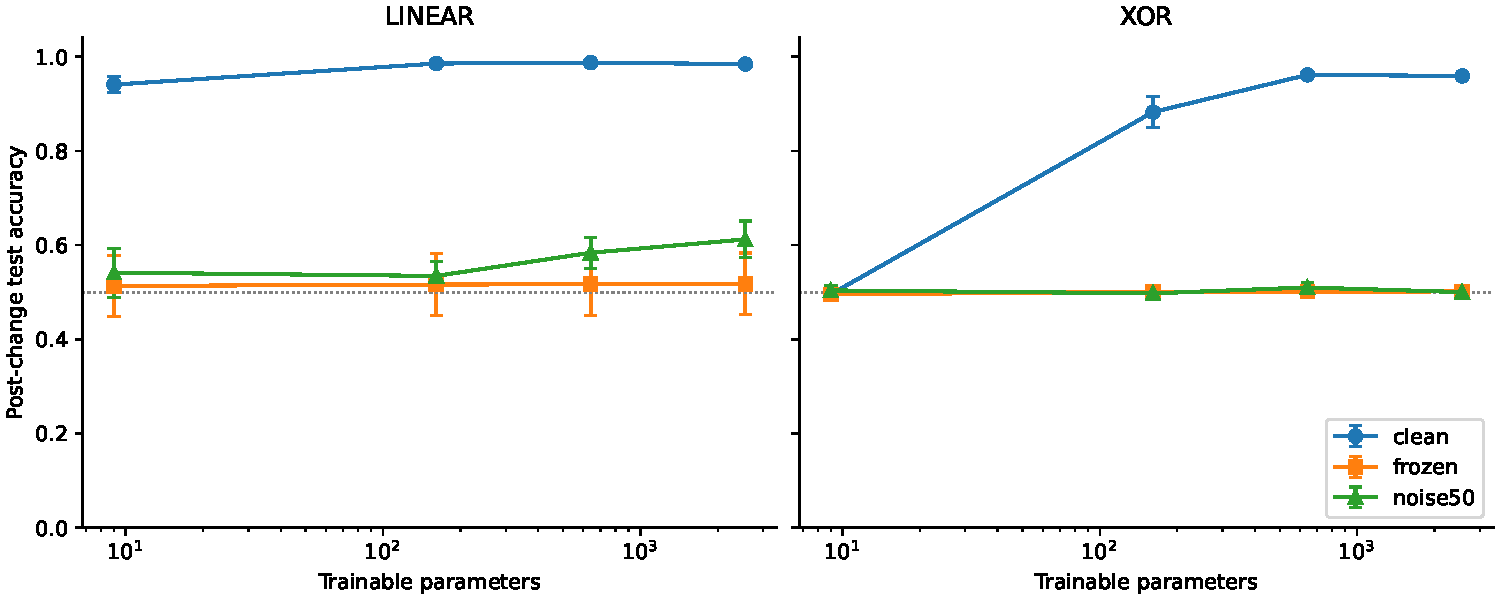
\includegraphics[width=\textwidth]{results/study-a-v1/capacity-feedback.pdf}
\caption{Capacity and feedback jointly determine observed accuracy. Error
bars are descriptive 95\% t intervals across 20 seeds. The dotted line is
chance accuracy; noisy feedback can coexist with information retained from
warmup, so individual noisy outcomes need not equal chance.}
\end{figure}

At an equal adaptation arithmetic proxy, the small model's 256 updates and
the largest model's 16 updates both cost 7,077,888 proxy FLOPs. The small
model leads by 35.09 points on linear tasks and 35.73 on XOR. However, it
receives sixteen times as many new examples, while the large model's warmup
cost is sixteen times greater. This is a particular compute/information trade,
not an isolated causal effect of feedback-loop efficiency or a scaling law.

\subsection{Feedback variations, transfer, and retention}
For the 161-parameter model, clean, 25\% corruption, and 50\% corruption yield
98.53\%, 92.88\%, and 53.45\% accuracy on linear tasks and 88.23\%, 70.95\%,
and 49.75\% on XOR. Inverted feedback yields 1.50\% and 12.01\% respectively.
More updates can reinforce the wrong target when the update rule assumes
trusted labels.

Delayed feedback reaches 98.52\% and 85.45\% at the online endpoint. After
flushing, its scores and final training losses equal clean feedback for every
seed and capacity. This equality is a correctness check for ordered updates,
not an additional empirical discovery about latency.

\begin{figure}[ht]
\centering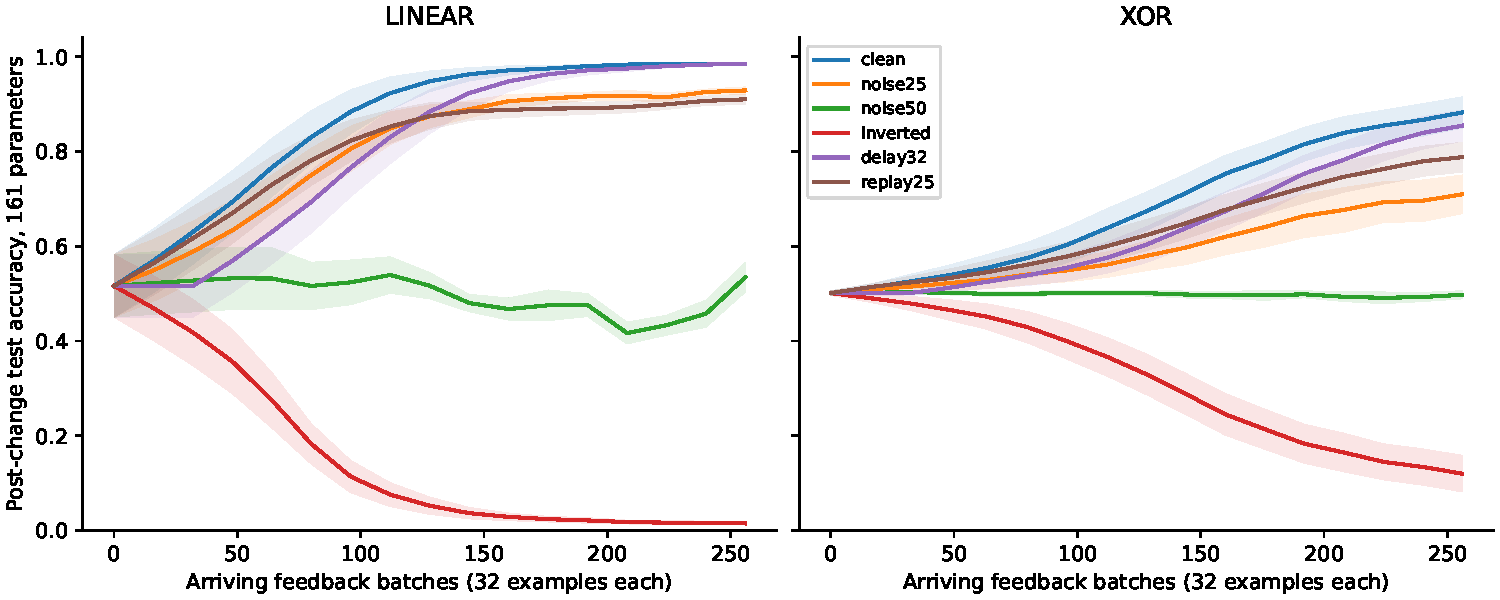
\includegraphics[width=\textwidth]{results/study-a-v1/learning-curves.pdf}
\caption{The same 161-parameter learner under six update conditions. Shading
shows descriptive 95\% seed-level intervals at fixed arrival checkpoints.}
\end{figure}

Clean small-model uniform-input accuracy is 98.64\% for linear rules and
90.95\% for XOR. This is distribution transfer within the same known rule
family, not transfer to an unrelated task. Old-rule accuracy after clean
adaptation is 51.76\% and 53.21\%. Replay raises these to 60.29\% and
65.03\% while lowering new-rule accuracy to 91.00\% and 78.79\%.
Because rules may conflict without a task identifier, this is an adaptation--
retention tradeoff; perfect performance on both is not always possible.

\subsection{Limitations and pending evidence}
The data are small, synthetic, and fully specified; labels are free and exact
except when deliberately corrupted. We test no autonomous information
acquisition, long-horizon reward, natural language, meta-learning, or durable
cross-domain skill accumulation. The optimizer schedule is fixed rather than
separately optimized by capacity, so its outcomes are conditional on that
schedule. A model-size threshold for arbitrary intelligence is not identified.

The prospective Study B compares four released Qwen2.5 model sizes on hidden
command mappings, true versus guessed feedback, explicit-rule controls, and
parameter updates tested without retained demonstrations. Its results are
not yet included here. Even positive results would require broader real-world
evaluation before supporting the original expansive hypothesis.

\section{Conclusion}
Under controlled task changes, feedback lets small neural learners recover
capability unavailable to frozen models. Capacity still matters when both
models learn, and reliable information and a suitable update mechanism remain
necessary. The present evidence supports conditional feedback-driven
adaptation. It does not establish that feedback alone explains intelligence
or that parameter scaling is an incorrect research direction.

\begin{thebibliography}{11}
\bibitem{vaswani} A. Vaswani et al. Attention Is All You Need. NeurIPS, 2017.
\url{https://arxiv.org/abs/1706.03762}.
\bibitem{kaplan} J. Kaplan et al. Scaling Laws for Neural Language Models. 2020.
\url{https://arxiv.org/abs/2001.08361}.
\bibitem{hoffmann} J. Hoffmann et al. Training Compute-Optimal Large Language Models. 2022.
\url{https://arxiv.org/abs/2203.15556}.
\bibitem{chen} H. Chen et al. Feedback is all you need: from ChatGPT to autonomous driving. 2023.
\url{https://doi.org/10.1007/s11432-023-3740-x}. Bibliographic metadata verified;
full-text argument not assessed in this version.
\bibitem{duan} Y. Duan et al. RL$^2$: Fast Reinforcement Learning via Slow Reinforcement Learning. 2016.
\url{https://arxiv.org/abs/1611.02779}.
\bibitem{laskin} M. Laskin et al. In-context Reinforcement Learning with Algorithm Distillation. 2022.
\url{https://arxiv.org/abs/2210.14215}.
\bibitem{shinn} N. Shinn et al. Reflexion: Language Agents with Verbal Reinforcement Learning. 2023.
\url{https://arxiv.org/abs/2303.11366}.
\bibitem{madaan} A. Madaan et al. Self-Refine: Iterative Refinement with Self-Feedback. 2023.
\url{https://arxiv.org/abs/2303.17651}.
\bibitem{huang} J. Huang et al. Large Language Models Cannot Self-Correct Reasoning Yet. 2023.
\url{https://arxiv.org/abs/2310.01798}.
\bibitem{snell} C. Snell et al. Scaling LLM Test-Time Compute Optimally can be More Effective than Scaling Model Parameters. 2024.
\url{https://arxiv.org/abs/2408.03314}.
\end{thebibliography}
\end{document}
